\chapter{Bullseye: A parallel targeted facet imager}
\section{Design objectives}
The primary design objectives of this work is to build a scalable parallel facet-based imager. A full deconvolution pipeline is currently out of scope, instead 
the focus is on accelerating the gridding step, since this step will be called on multiple times in a major-minor cycle deconvolution pipeline as discussed in 
chapter \ref{chapter_synthesis}. To this end we will focus on comparing performance between parallel CPU-based resampling and a GPU approach.
\section{Architecture}
We've decided to split up the our implementation into two major components:
\begin{enumerate}
 \item A front-end program dealing with the logic of reading in measurement data, dealing with user options, overall program flow and image finalization.
 \item A set of back-end libraries that implement a common interface and house the resampling and transformation routines. The resampling routines include options to resample multiple
 correlations and enable faceting and w-projection logic.
\end{enumerate}

The architecture above allows us to easily swap out one set of resampling routines for another and to compare between CPU and GPU-based implementations. Figure~\ref{fig_arch} shows
the major components of our imager, along with several major dependencies. 
\begin{figure}[h]
  \begin{mdframed}
    \centering
    \begin{subfigure}[b]{0.66\textwidth}
      \centering
      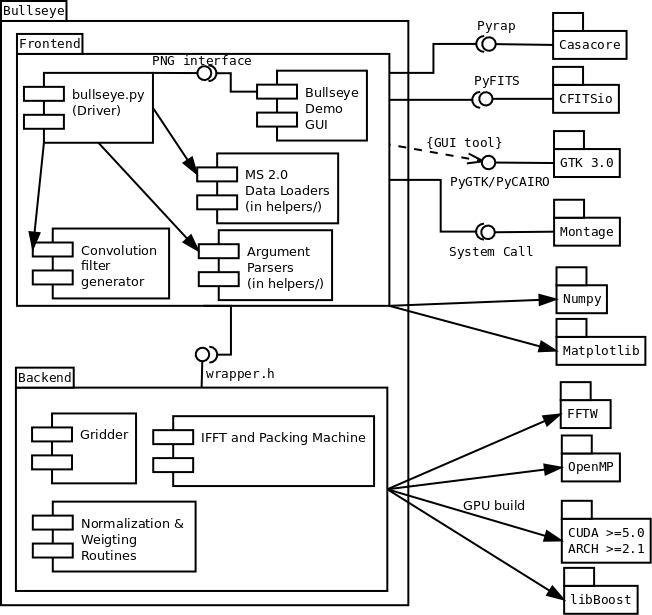
\includegraphics[width=\textwidth]{images/bullseye_arch.png}
      \caption{}
    \end{subfigure}  
    \caption[Bullseye Architecture]{The front end of the solution contains a commandline utility that has very similar options to that provided in other imagers, such as lwimager.
    Included with it are modules required to generate the w-projection convolution functions and a prototype graphical interface illustrating targeted faceting. The backend consists
    of the resampling routines along with routines to do fourier shifting, inversion and normalization on a set of facets that may each contain multiple spectral images.}
    \label{fig_arch}
  \end{mdframed}
\end{figure}
\section{Normal workflow}
During imaging the user will supply a set of facet centre coordinates, number of facets splitting the sky (or both), along with a measurements database and outputs a set of facet images that can optionally
be recombined with the astronomical mosaicking package, Montage \cite{jacob2004montage}.

Program flow is indicated in Figure~\ref{fig_workflow}. The resampling and fourier inversion step may include sampling and transforming the sampling function.
The latter requires that all measurements are set to unity and a PSF is synthesized for each facet image. Additionally 
each facet may have resampling grids allocated for multiple correlations and spectral bands, and can therefore be facet cubes 
instead of simple 2D images. 

The fourier inversion step also entails shifting each of the facet grids such that the base uv-frequency of each grid
is located in the middle of the grids, thus shifting the image phase centre to the middle of each of the images.
\begin{figure}[ht!]
 \begin{mdframed}
 \centering
  \begin{tikzpicture}[node distance=4.5cm]
    \node (start) [start] {};
    \node (data) [draw,trapezium,trapezium left angle=70,trapezium right angle=-70,maximum width=1cm,right of=start] {%
							      \begin{varwidth}{10em}
								Facet coordinates, 
								image sizes, 
								channel selection
								and input measurement databases
							      \end{varwidth}};
    \node (readms) [process, right of=data] {Read measurements and meta data};
    \node (resampling) [process, below of=readms] {Convolutional resampling};
    \node (fft) [process, left of=resampling] {Shift, IFFT and normalize};
    \node (output) [draw,trapezium,trapezium left angle=70,trapezium right angle=-70,maximum width=1cm,left of=fft] {%
							      \begin{varwidth}{10em}
								Output to FITS images
							      \end{varwidth}};
    \node (stop) [stop, left of=output] {};
    
    \draw [rarrow] (start) -- (data);
    \draw [rarrow] (data) -- (readms);
    \draw [rarrow] (readms) -- (resampling);
    \draw [rarrow] (resampling) -- (fft);
    \draw [rarrow] (fft) -- (output);
    \draw [rarrow] (output) -- (stop);
  \end{tikzpicture}
 \caption[Imaging workflow]{This diagram shows the major steps involved in the synthesis process. The convolutional resampling step includes
 faceting transforms and w-projection logic.}
 \label{fig_workflow}
 \end{mdframed}
\end{figure}
\section{Input/Output formats}
\subsection{NRAO Measurement Set 2.0}
The Measurement Set standard \cite{ms10,ms20} is an AIPS++ (later CASA) database format containing telescope observation data, 
along with observation metadata. Correlated observation data is stored in a ``MAIN'' table, along with uvw coordinates, antenna ids, 
timestamp information, weighting and flagging information, along with foreign keys to subtables with meta data to the observation. The 
metadata describes everything from the antenna positions and mounts to feeds, spectral window descriptions and the observed fields.

Each row in the MAIN table contains measurements for a particular spectral band and may contain multiple correlations per spectral channel. Each
row contains $N_\text{channel}\times N_\text{correlation}$ measurements. The rows is not necessarily 
ordered by either baseline, time or antenna IDs by default and in total the Measurement Set MAIN table
will contain $N_\text{baseline}\times N_\text{timestamp}$ rows, including autocorrelated antennas. It is worth noting 
that during flagging and calibration some rows may be deleted from the Measurement Set.

\subsection{The Flexible Image Transport System}
\section{Targeted faceting and image mosaicking options}
\section{Continuum imaging vs. spectral line imaging}
\section{Work distribution strategies considered}
\subsection{CPU}
\subsection{GPU}